\documentclass[12pt,a4paper]{article}

% ===== Codificación y español =====
\usepackage[utf8]{inputenc}
\usepackage[T1]{fontenc}
\usepackage[spanish, es-tabla]{babel}

% ===== Márgenes y gráficos =====
\usepackage{geometry}
\geometry{margin=2.5cm}
\usepackage{graphicx}
\usepackage{float}        % [H] para fijar figuras/tablas
\usepackage{subcaption}   % subfiguras
\usepackage{booktabs}     % tablas más bonitas

% ===== Hipervínculos y referencias =====
\usepackage{hyperref}
\hypersetup{
  colorlinks=true,
  linkcolor=black,
  citecolor=black,
  urlcolor=blue
}

\usepackage{siunitx}
\sisetup{
  output-decimal-marker = {.}, % decimal con punto
  group-separator = {,},       % miles con coma
  group-minimum-digits = 4,
  group-digits = integer,
  table-number-alignment = center,
  round-mode = places,
  detect-all = true            % ignora configuraciones de babel
}

% Ayuda al manejo de tablas
\usepackage{tabularx}
\usepackage{adjustbox}
\usepackage{longtable}

% cleveref mejora \ref: escribe "Figura 1", "Tabla 2", etc.
\usepackage[capitalise,noabbrev]{cleveref}

% Ajuste de nombres en cleveref
\crefname{figure}{figura}{figuras}
\Crefname{figure}{Figura}{Figuras}
\crefname{subfigure}{subfigura}{subfiguras}
\Crefname{subfigure}{Subfigura}{Subfiguras}
\crefname{table}{tabla}{tablas}
\Crefname{table}{Tabla}{Tablas}
\crefname{equation}{ecuación}{ecuaciones}
\Crefname{equation}{Ecuación}{Ecuaciones}
\crefname{section}{sección}{secciones}
\Crefname{section}{Sección}{Secciones}

% Listas más controlables
\usepackage{enumitem}

\graphicspath{{figures/}}

% ===== Título y autoría =====
\title{\textbf{\textit{"Playing"} con diferentes clasificadores y datasets}}
\author{Haessler Joan Ortiz Moncada \\[0.5cm]
        Universidad Distrital Francisco José de Caldas \\
        Facultad de Ingeniería \\
        Curso: Big Data}
\date{\today}

\begin{document}

\maketitle

\section{Introducción}
Este documento presenta el desarrollo del taller \#2 del curso de Construcción de Pruebas de Software. 
Su propósito es documentar los hallazgos de la implementación de la recursión en métodos de suma, 
multiplicación y cálculo del factorial, así como su integración, utilizando el lenguaje de programación 
\textbf{Java}. Además, se aplican pruebas unitarias a estos métodos, se publica el proyecto en \textbf{GitHub} 
y se automatiza la ejecución de dichas pruebas ante cada \textit{push} y \textit{pull request}. Por último, 
el informe explica brevemente qué es Postman, para qué sirve y muestra algunos ejemplos de uso.

\section{Metodología}
El proyecto Java con la implementación recursiva se desarrolló en el Entorno de Desarrollo Integrado 
(IDE, por sus siglas en inglés) \textbf{IntelliJ IDEA}, aprovechando que ya contaba con este software y con 
el Kit de Desarrollo de Java (JDK) instalado en la máquina local. Para el diseño, ejecución y documentación 
de las pruebas se empleó el \textit{framework} \textbf{JUnit}. El control de versiones y la publicación del 
proyecto en un repositorio remoto se realizaron con \textbf{Git} y \textbf{GitHub}. Finalmente, la automatización 
de las pruebas unitarias se configuró mediante un archivo \texttt{.yml} para que la sección \textbf{Actions} de 
GitHub ejecute las pruebas en cada \textit{push} y \textit{pull request}.

Respecto a Postman se probaron los métodos \textit{http} clásicos (\textit{GET, POST, PUT, DELETE}) mediante 
solicitudes a una Interfaz de Programación de Aplicaciones (API, por sus siglas en inglés) pública.

\section{Desarrollo}

\subsection{Recursión}
Se diseñó una clase sencilla con tres funciones recursivas: una que suma, otra que multiplica apoyándose en la 
suma, y la del factorial que usa la multiplicación. Se impuso un tope claro: sólo se calcula hasta \(10!\), si se 
excede o se ingresan negativos, se avisa con una excepción. La idea fue mantener la ``recursividad en capas'' 
sin depender de un operador de multiplicación directo dentro del factorial.

\subsection{JUnit}
Se craron pruebas unitarias con JUnit 5 y, para no repetir la invocación de las preubas, se usaron pruebas parametrizadas: 
se escribe una sola prueba y se pasan varias filas de datos. Se probaron los sigueintes aspectos:

\begin{enumerate}
  \item \textbf{Casos correctos}: valores típicos y casos base (por ejemplo, factoriales de 0 a 10).
  \item \textbf{Propiedades}: se comprobó que la multiplicación no depende del orden de los factores (conmutatividad).
  \item \textbf{Errores esperados}: se verificó que, cuando toca, se lance la excepción correcta (por ejemplo, si \(n>10\) o si hay negativos).
\end{enumerate}

La \Cref{fig:str_project} muestra como luce el proyecto Java que se construyó.

\begin{figure}[h]
  \centering
  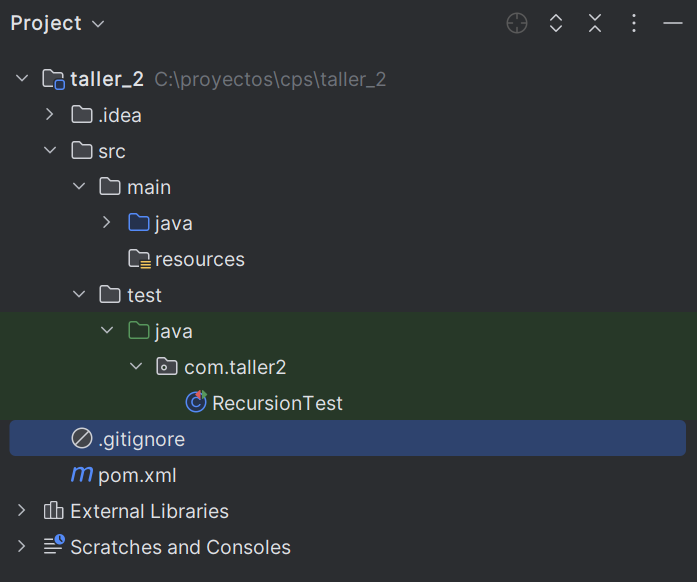
\includegraphics[width=\textwidth]{str_project.png}
  \caption{Estructura proyecto Java.}
  \label{fig:str_project}
\end{figure}

\subsection{GitHub Actions}
Una vez se hizo \textit{push} del proyecto Java al repositorio de GitHub \href{https://github.com/HaesslerOrtiz/cps}{cps\_repositorio}, 
se agregó un archivo \texttt{workflow} en la ruta \texttt{.github/workflows/ci.yml} en la raiz del repositorio, esto con la intención de 
generar la automatización de las pruebas al proyecto Java realizado. Con la creación de este archivo se logró lo siguiente:

\begin{enumerate}
  \item Se dispara solo en cada \textit{push} y en cada \textit{pull request}.
  \item Prepara y ejecuta los tests de \texttt{taller\_2}.
  \item Publica los reportes de pruebas como artefactos en la pestaña \textit{Actions}.
\end{enumerate}

La \Cref{fig:actions} muestra como luce la estructura del proyecto cargado y el archivo \texttt{.yml}.

\begin{figure}[H]
  \centering
  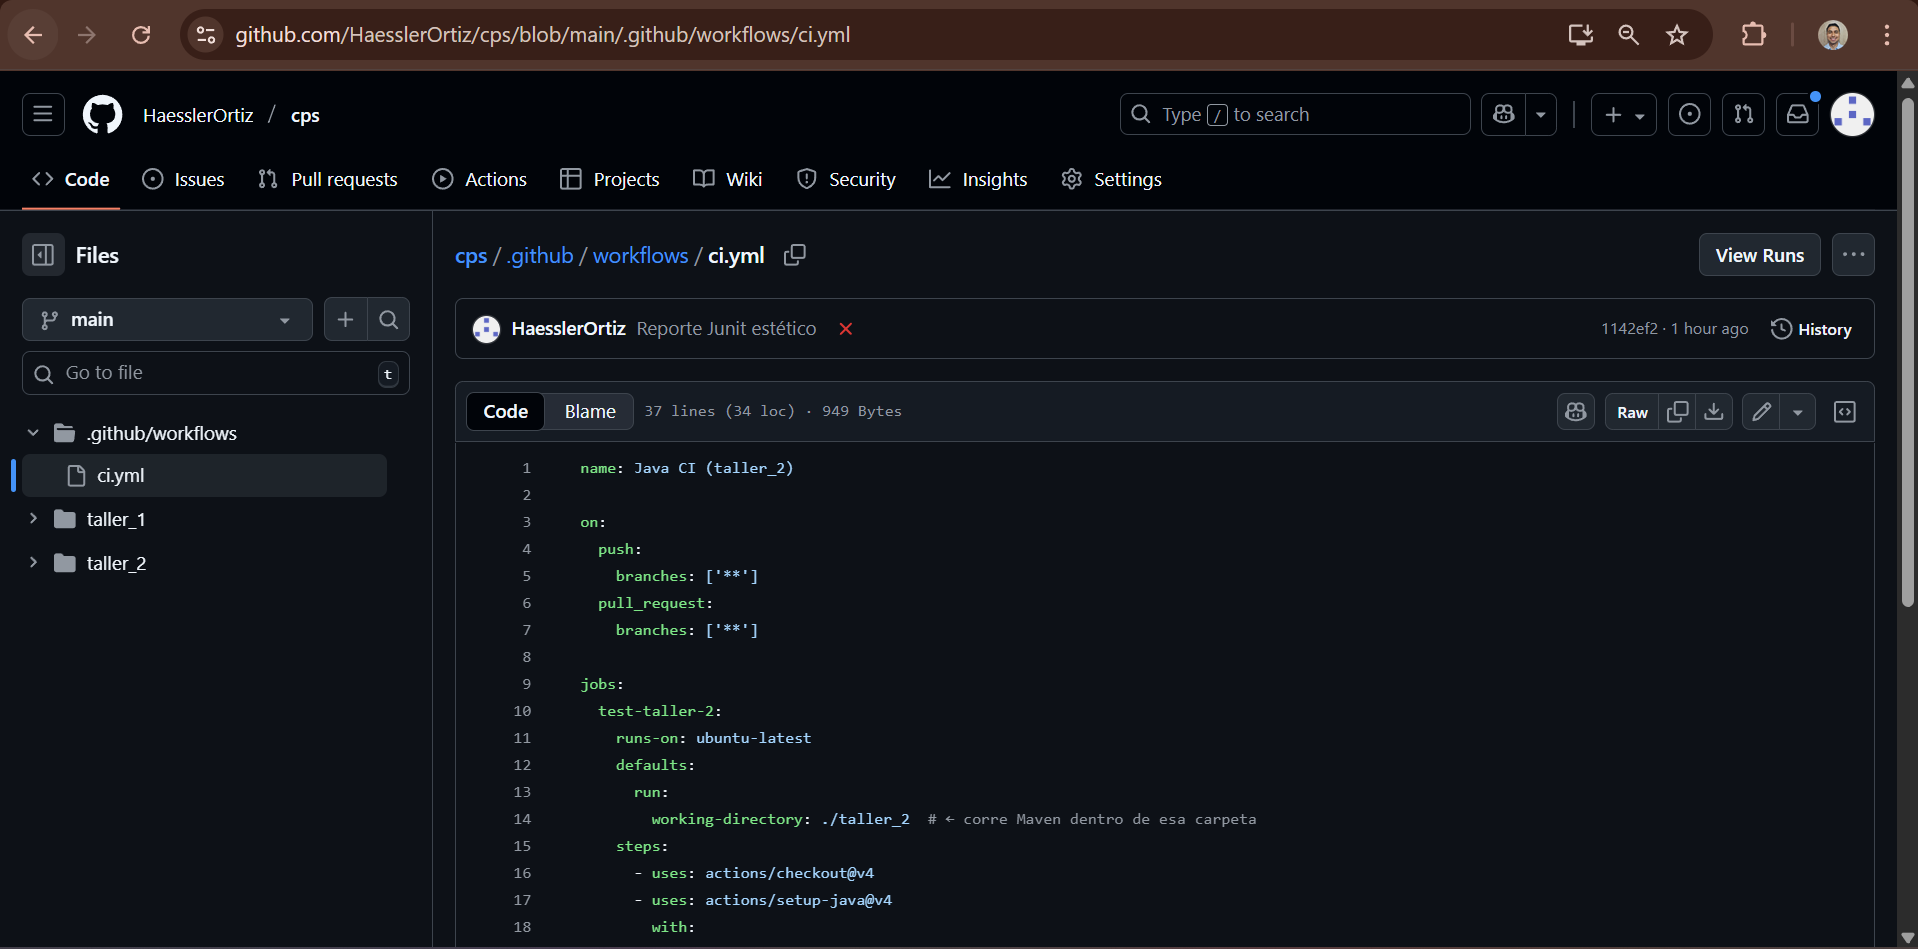
\includegraphics[width=\textwidth]{actions.png}
  \caption{Estructura proyecto Java.}
  \label{fig:actions}
\end{figure}

En cuanto a los resultados, se detectó el fallo de algunos \textit{tests} (aunque la mayoría de las pruebas pasaron). 
A partir de los \textit{logs}, la causa probable es una profundidad de recursión excesiva al calcular el factorial para 
ciertos valores de entrada, lo que deriva en errores de ejecución (p.~ej., \textit{stack overflow}). Como 
acciones de mejora, conviene simplificar la implementación (por ejemplo, adoptar una versión iterativa), validar 
el dominio de entrada (solo $n \geq 0$) y limitar el tamaño máximo permitido para $n$. La \Cref{fig:test} muestra 
el reporte generado por \texttt{GitHub Actions}.

\begin{figure}[H]
  \centering
  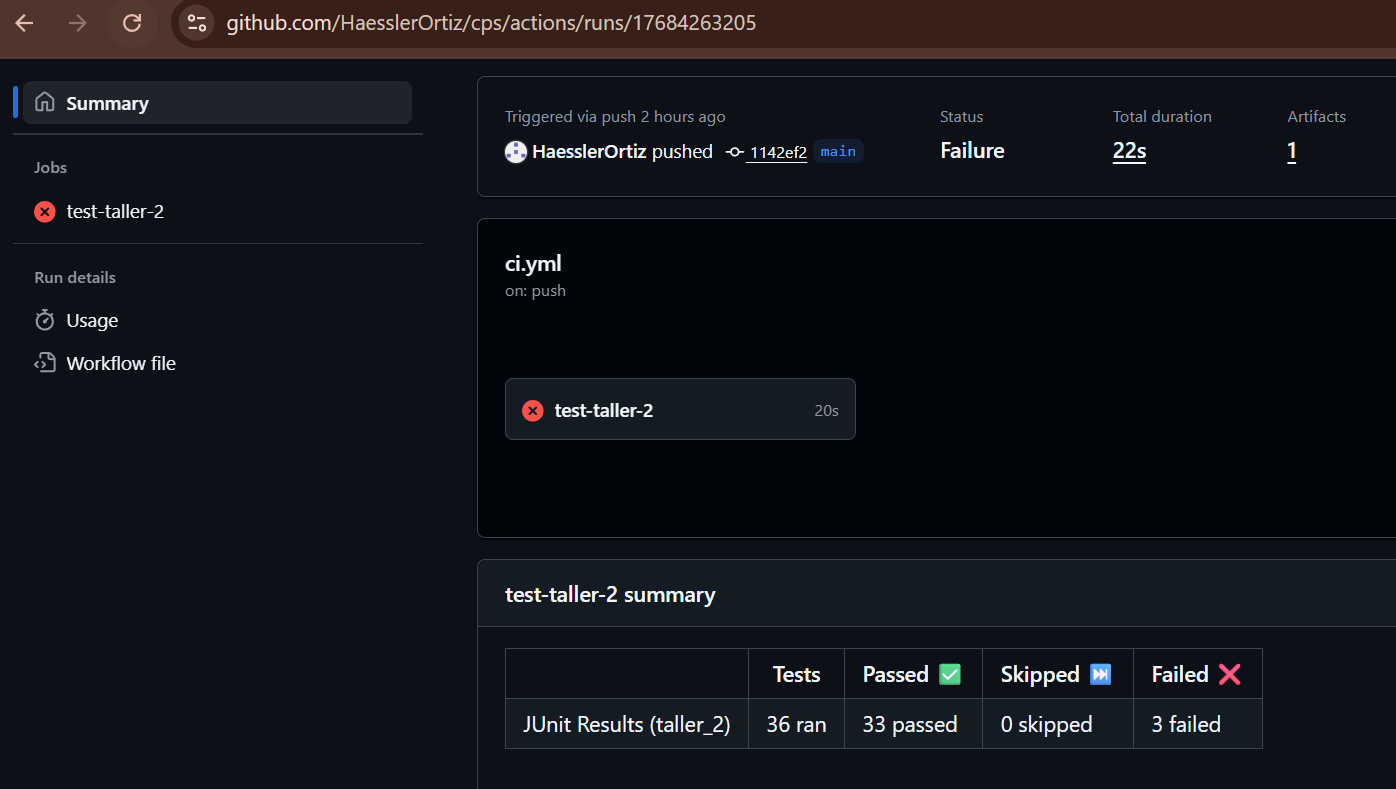
\includegraphics[width=\textwidth]{test.png}
  \caption{Reporte GitHub Actions.}
  \label{fig:test}
\end{figure}

El archivo \texttt{.yml} desarrollado, fue sugerida por la Inteligencia Artificial (IA) \textbf{ChatGPT}.

\subsection{Postman}
Postman es un programa que permite enviar preguntas a un servicio en internet y ver lo que ese servicio retorna. 
Es como una ventana sencilla para conversar con esos servicios y entender qué devuelven. Postman permite lo siguiente:

\begin{enumerate}
  \item Comprobar rápidamente si un servicio en línea está funcionando.
  \item Probar cómo responde cuando se envías datos.
  \item Guardar y repetir pruebas sin volver a escribir todo cada vez.
  \item Compartir esas pruebas con otras personas.
  \item Detectar errores de un servicio.
\end{enumerate}

Después de crear una cuenta (con mi correo Gmail) e iniciar una sesión en Postman, me apareció la siguiente interfaz:

\begin{figure}[H]
  \centering
  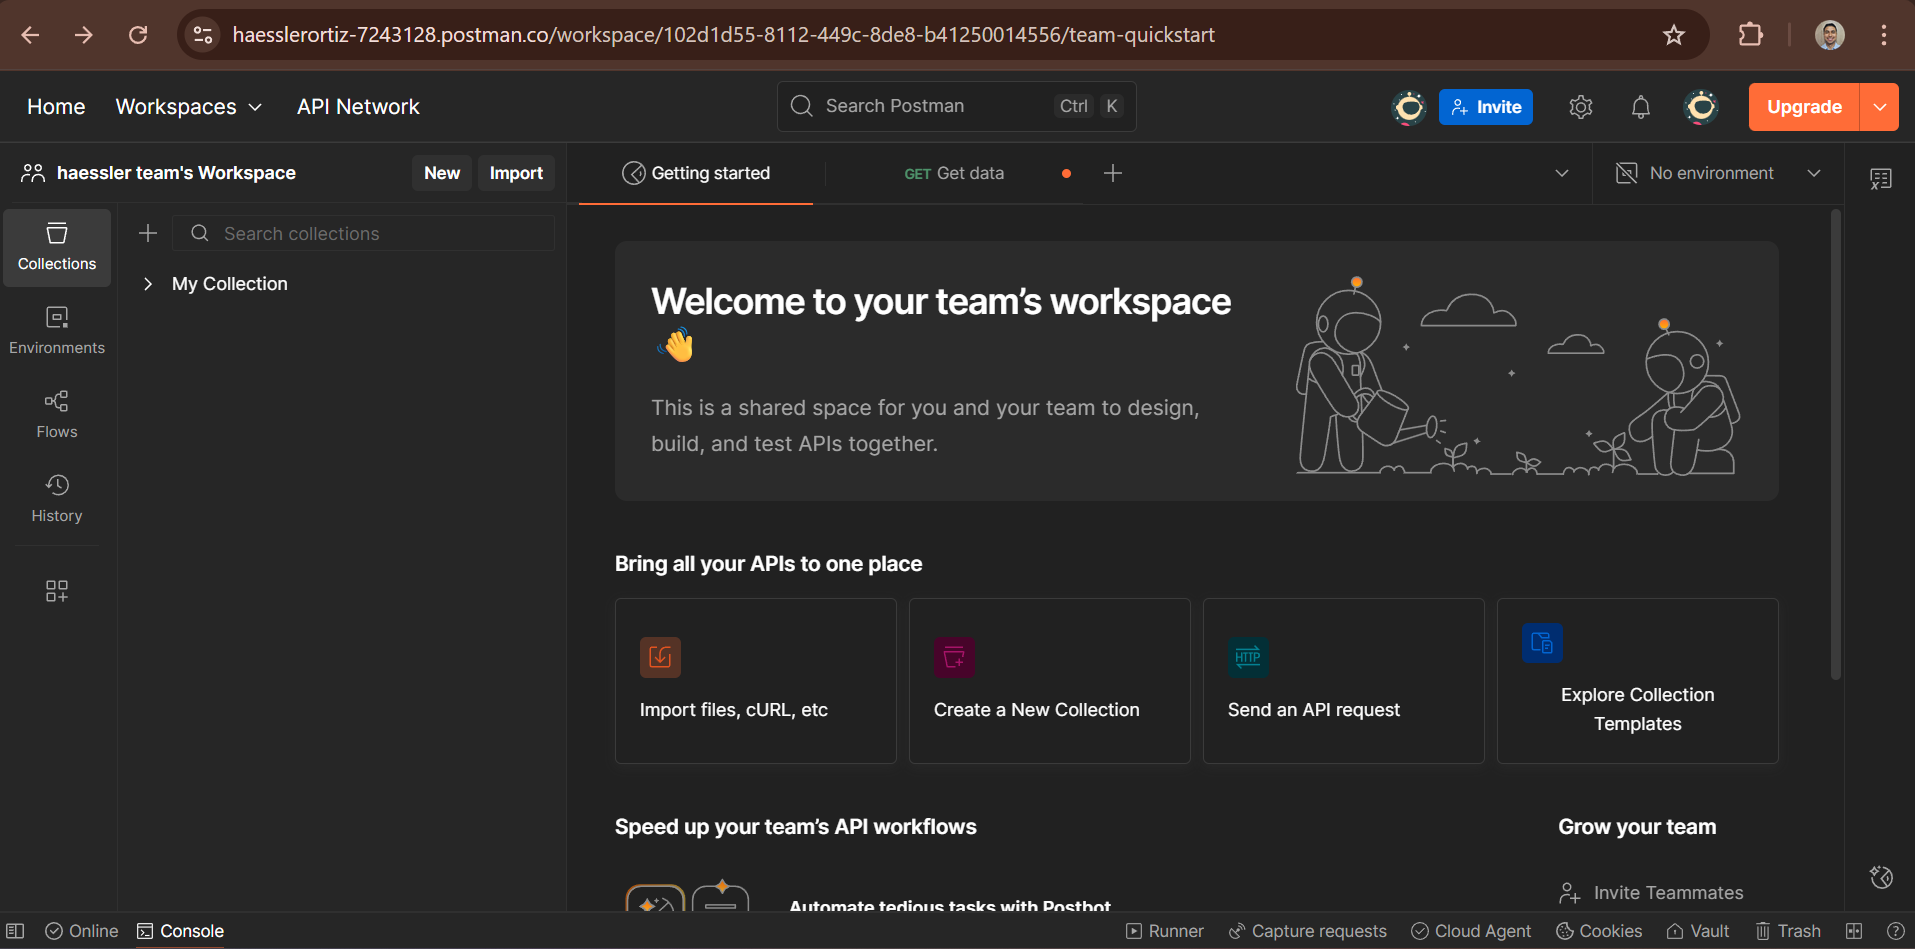
\includegraphics[width=\textwidth]{postman.png}
  \caption{Reporte GitHub Actions.}
  \label{fig:postman}
\end{figure}

Una vez allí probé los métodos clásicos \textit{http}, en la API pública \href{https://jsonplaceholder.typicode.com}. 
Se obtuvieron los sigueintes resultados:

\begin{itemize}
  \item \textbf{GET.}
  Diligenciando el \textit{endpoint} \href{https://jsonplaceholder.typicode.com/posts/1} se obtuvo el siguiente resultado:

  \begin{figure}[H]
    \centering
    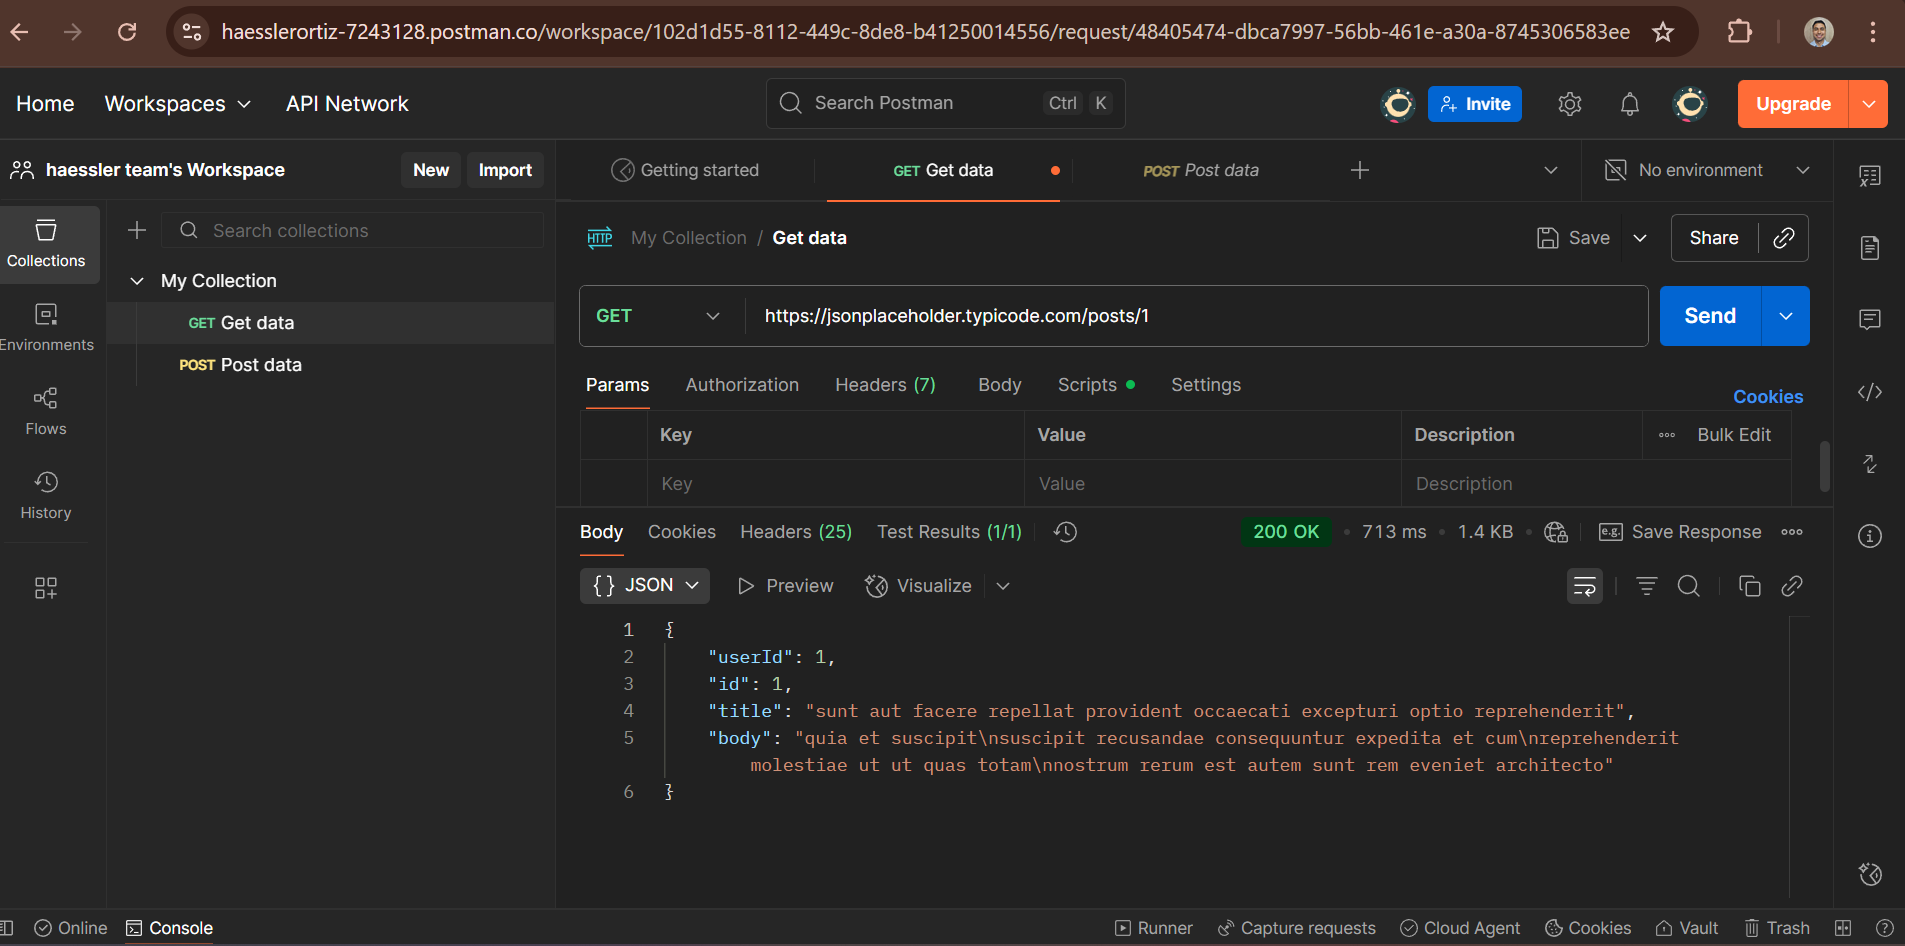
\includegraphics[width=\textwidth]{get.png}
    \caption{Solicitud GET.}
    \label{fig:get}
  \end{figure}

  La \Cref{fig:get} muestra el estado de la Transferencia de Estado Representacional (REST, por sus siglas en inglés) y el 
  contenido del Objeto con Notación \textit{JavaScript} (JSON, por sus siglas en inglés).
 
  \item \textbf{POST.}
  Diligenciando el \textit{endpoint} \href{https://jsonplaceholder.typicode.com/posts} y configurando el \textit{body} del 
  JSON (resaltado en amarillo en la \Cref{fig:post}) a enviar, se obtuvo lo siguiente:

  \begin{figure}[H]
    \centering
    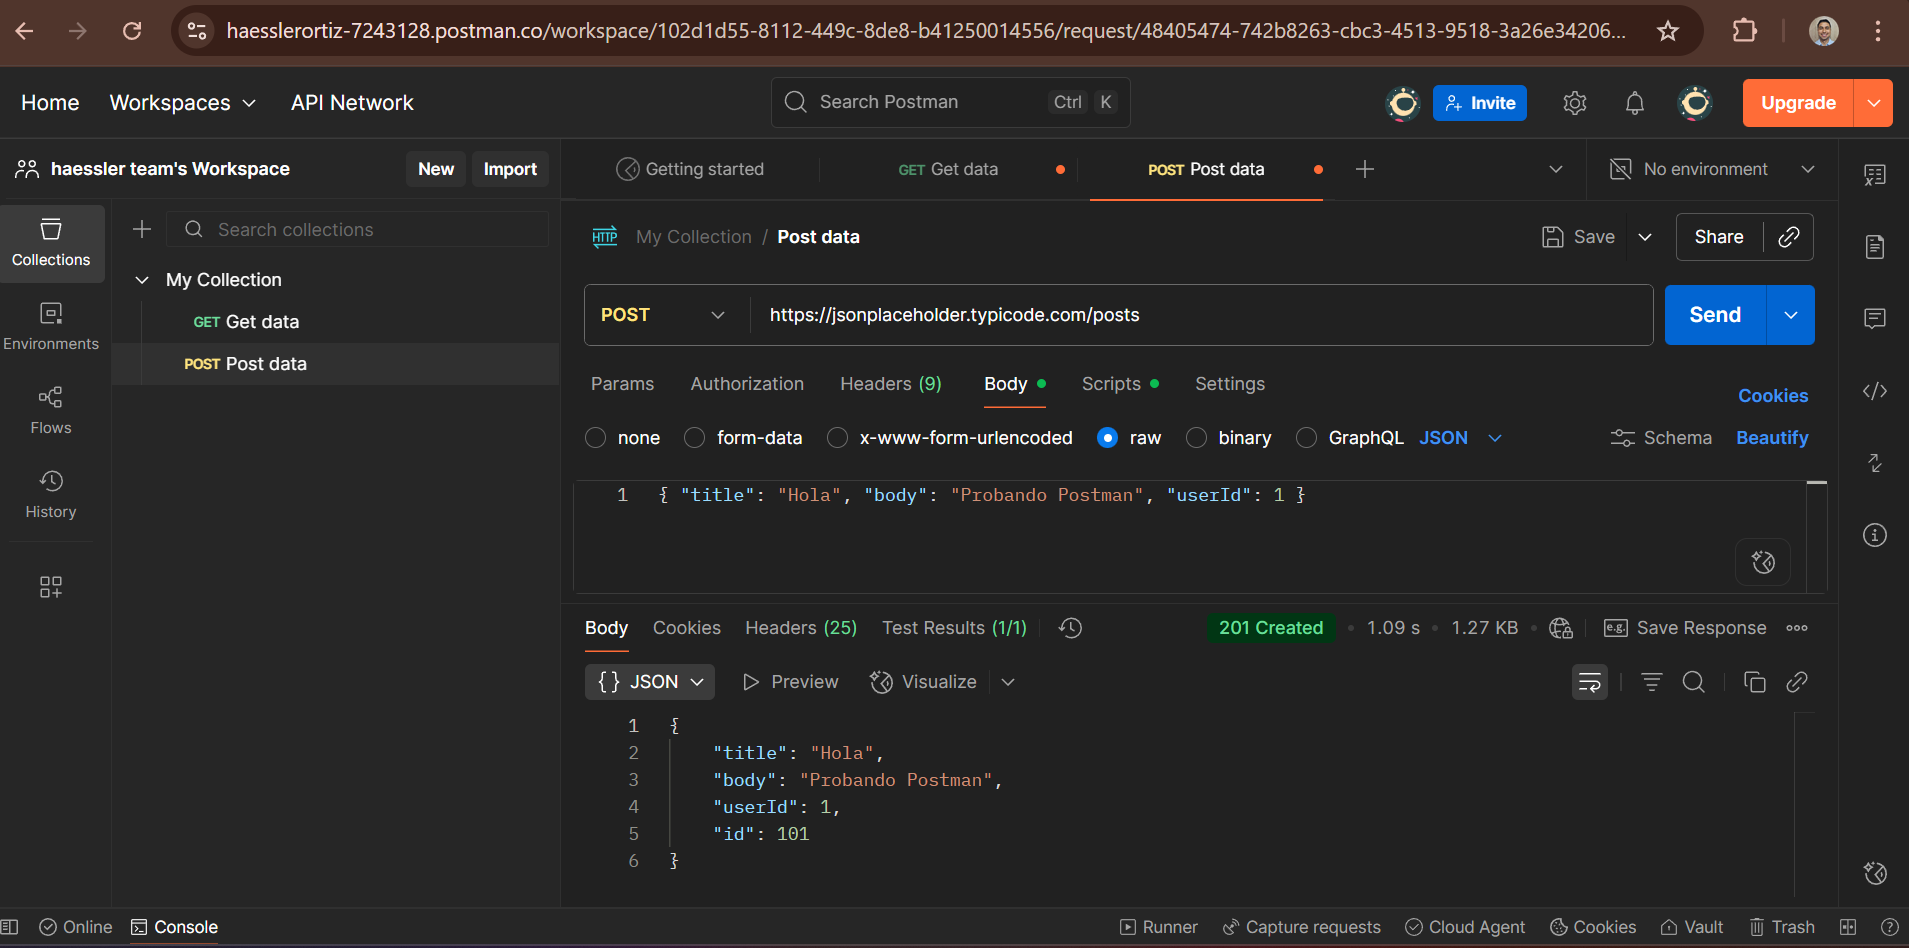
\includegraphics[width=\textwidth]{post.png}
    \caption{Solicitud POST.}
    \label{fig:post}
  \end{figure}

  \item \textbf{PUT.}
  Con un procedimiento similar al anterior, se actualizó el JSON que en la solicitud anterior se había generado. La \Cref{fig:put} 
  muestra el resultado:

  \begin{figure}[H]
    \centering
    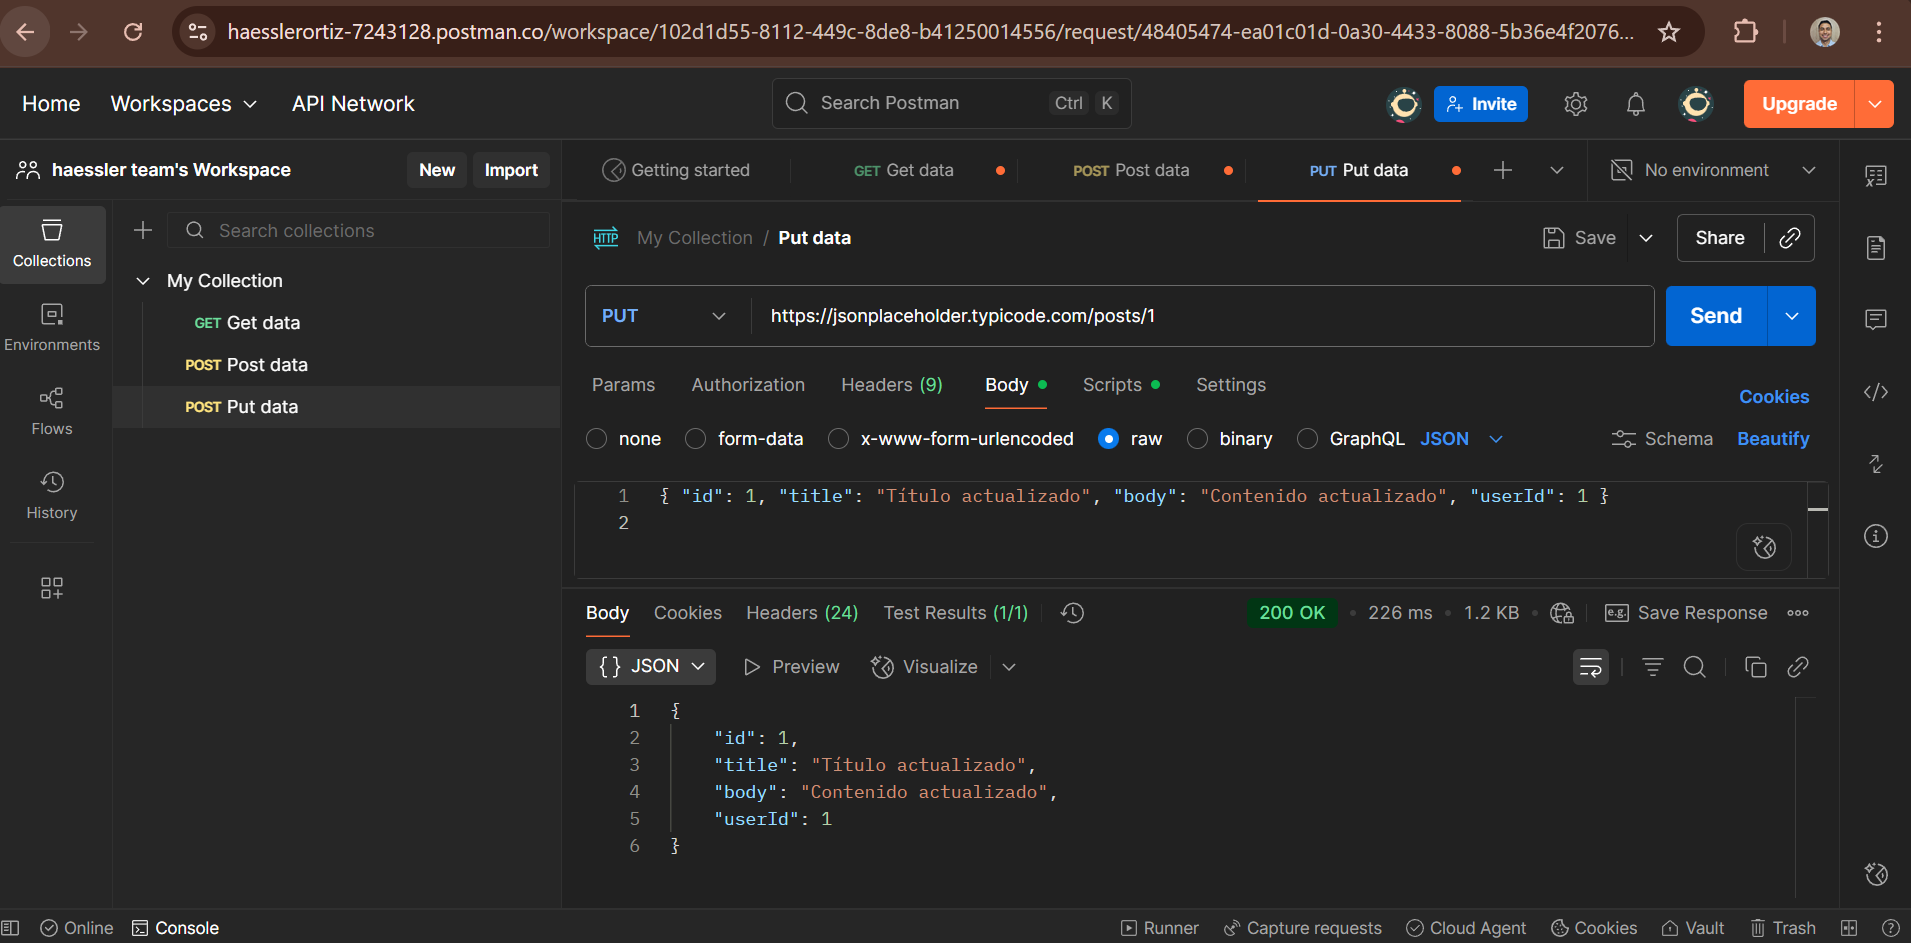
\includegraphics[width=\textwidth]{put.png}
    \caption{Solicitud PUT.}
    \label{fig:put}
  \end{figure}

  \item \textbf{DELETE.}
  Aquí lo que se hizo fue borrar el registro que reciéntemente modificamos. Se tuvo el siguiente resultado:

  \begin{figure}[H]
    \centering
    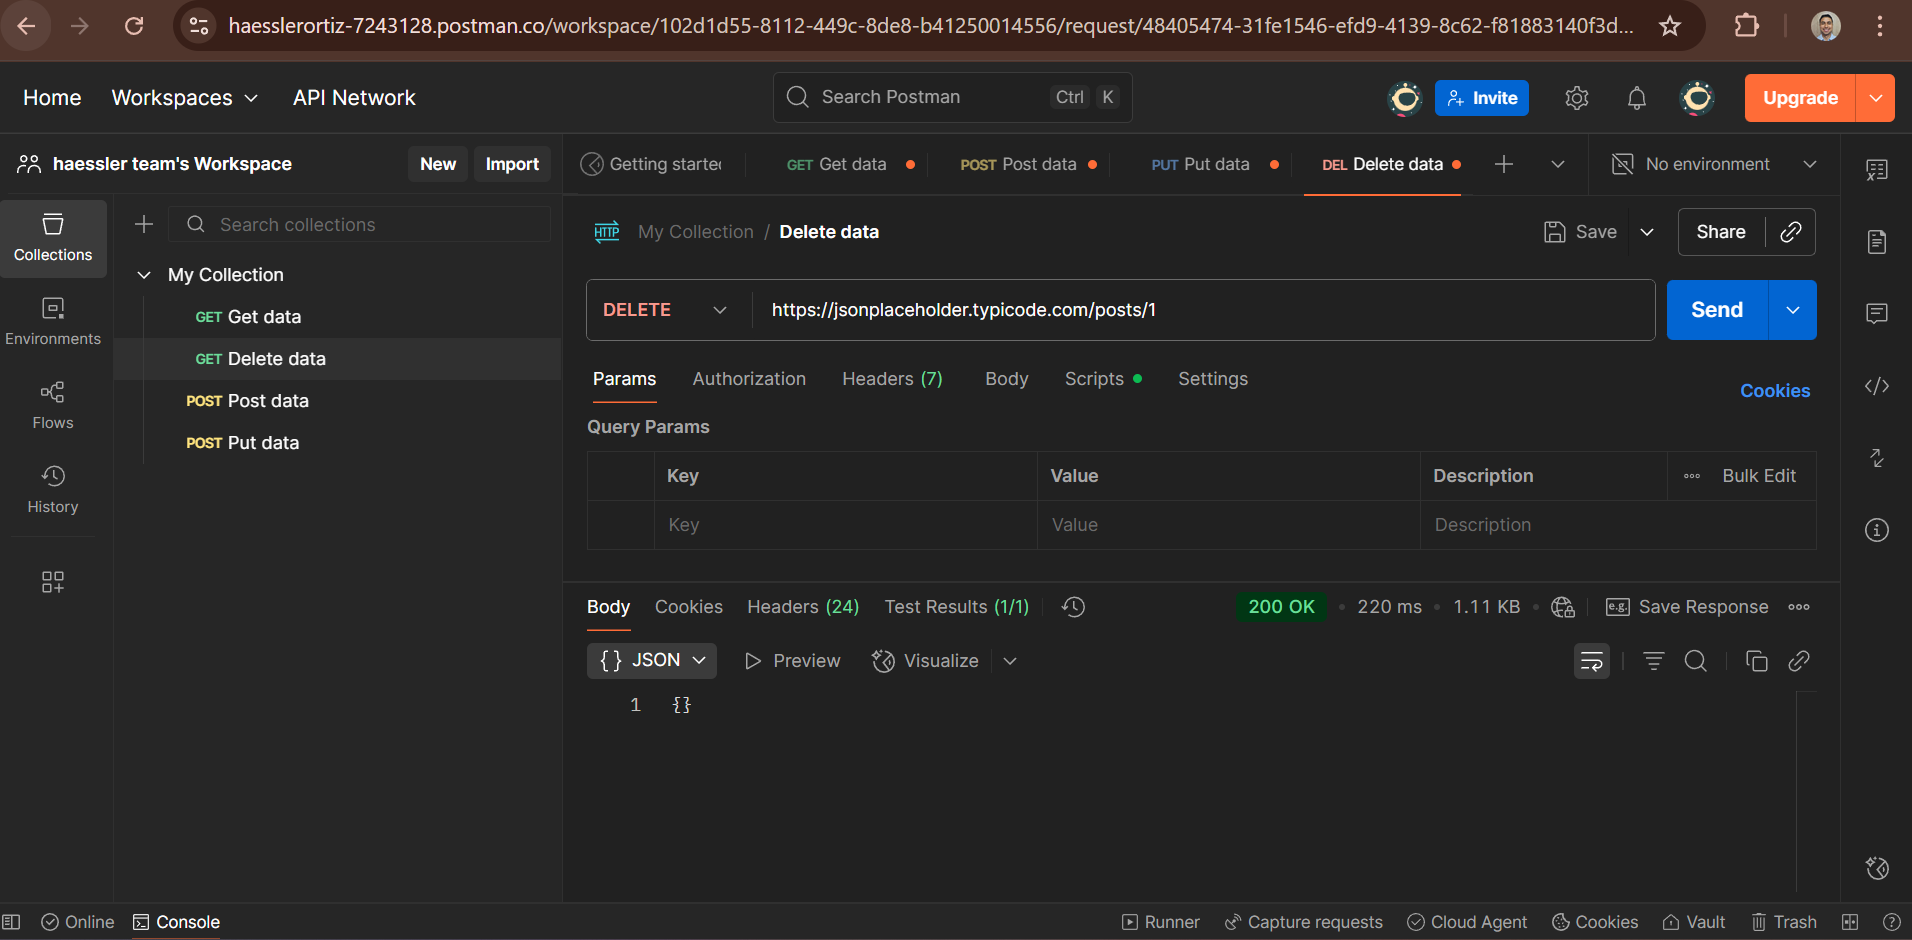
\includegraphics[width=\textwidth]{delete.png}
    \caption{Solicitud DELETE.}
    \label{fig:delete}
  \end{figure}

  La API aquí utilizada, fue sugerida por la Inteligencia Artificial (IA) \textbf{Gemini}.
\end{itemize}


\end{document}
